\section{\protein{Mad1}'s loop region is important to the SAC signaling activity \Latin{in vivo}}
\label{LoopDeletionSection}

We next sought to determine whether the loop region of \protein{Mad1} that likely enables the fold-back conformation is important to the SAC signaling activity \Latin{in vivo}. We integrated the expression cassette of either \protein{Mad1}-mNG or \protein{Mad1}\textDelta{}L-mNG into the genome of HeLa-A12 cells using Cre-\bacterialgene{lox} RMCE (see \myref{Cre-lox}). We then knocked down endogenous \protein{Mad1} in these cells using siRNAs that target the 3'-UTR of \gene{Mad1} \cite{siMAD1-3UTR} (henceforth collectively referred to as si\gene{Mad1}'s) and induced the expression of \protein{Mad1}(WT/\textDelta{}L)-mNG (si\gene{Mad1}-resistant due to the lack of the endogenous 3'-UTR) by doxycycline. Our genome-edited \gene{Mad1}-mNG HeLa-A12 cell line served as the reference for the endogenous level of \protein{Mad1} in live-cell fluorescence imaging.

We found out that knocking down \gene{Mad1} crippled the SAC signaling activity. However, cells with less than 10\% of the physiological level of \protein{Mad1} on average (estimated from the immunoblot in \myref{MAD1Rescue_WB}) still arrested in mitosis for hours when treated with \SI{100}{nM} nocodazole (only about two hours less than the control group with a physiological level of \protein{Mad1}). Increasing the dosage of si\gene{Mad1}'s did not further decrease the SAC activity, reinforcing that even a small pool of \protein{Mad1} could sustain a considerable level of SAC signaling activity.




\begin{figure}
    \centering
    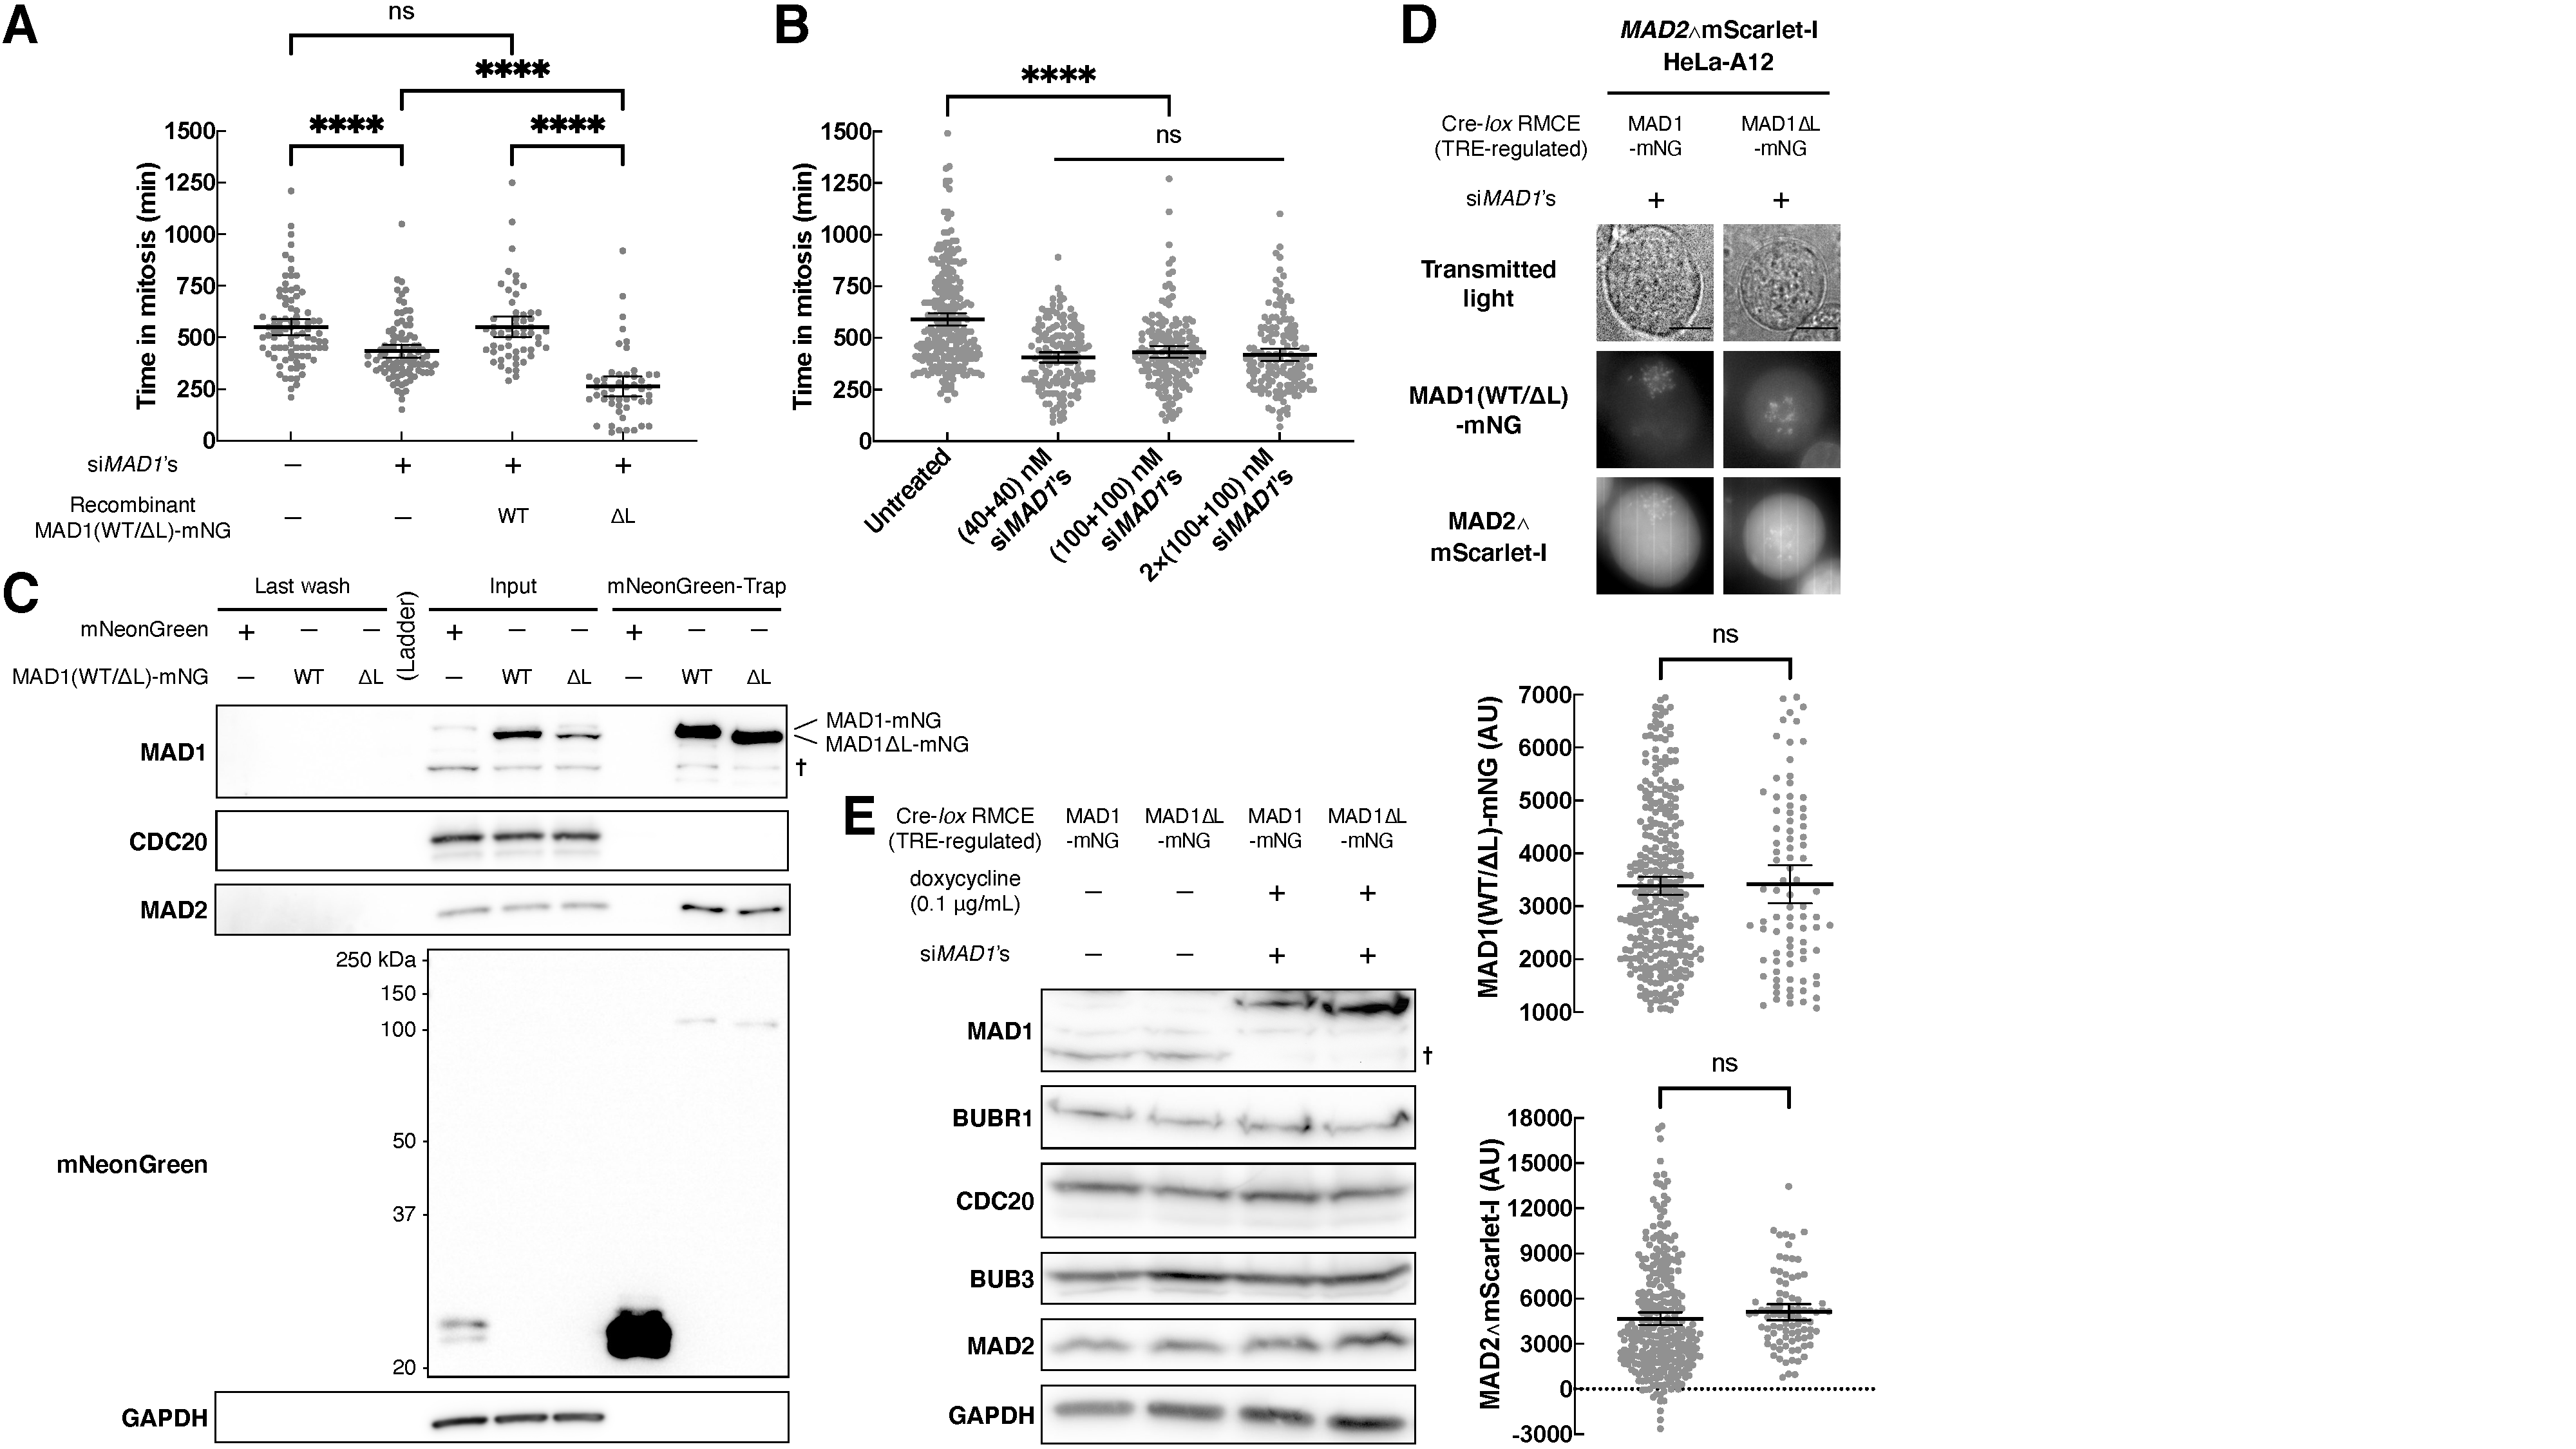
\includegraphics[trim={0 0 0 3cm},clip]{chapters/figures/MAD1Rescue.pdf}
    \phantomsubfiglabel{MAD1Rescue_Main} % subfigure A
    \phantomsubfiglabel{MAD1Rescue_LimitPushing} % subfigure B
    \phantomsubfiglabel{MAD1Rescue_HeterodimerizationWB} % subfigure C
    \phantomsubfiglabel{MAD1Rescue_Localization} % subfigure D
    \phantomsubfiglabel{MAD1Rescue_WB} % subfigure E
    \caption{\textbf{.}}
    \noindent\justifying 
    \label{MAD1Rescue}
\end{figure}


% by transfecting the cells with si\gene{Mad1}'s for two days
% we quantified the localization of \protein{Mad1}(wildtype/\textDelta{}L)-mNG and \protein{Mad2}$\wedge$mScarlet-I at signaling kinetochores by fluorescence imaging and quantified the expression level of other SAC proteins by immunoblotting. Genome-edited \gene{Mad2}$\wedge$mScarlet-I HeLa-A12 cells treated with si\gene{Mad1}'s and rescued by \protein{Mad1}(wildtype/\textDelta{}L)-mNG showed that no difference in the localization of either \protein{Mad1} or \protein{Mad2} at signaling kinetochores. The cellular abundance of some other SAC proteins like \protein{BubR1}, \protein{Cdc20}, and \protein{Bub3} was also not affected by the rescue experiment.

Surprisingly, \protein{Mad1}\textDelta{}L-mNG had impaired support for the SAC in a dominant-negative manner: cells treated with si\gene{Mad1}'s and rescued by a physiological level of \protein{Mad1}\textDelta{}L-mNG arrested in mitosis for a significantly shorter duration than cells which were not rescued. As a comparision, wildtype \protein{Mad1}-mNG fully restored the SAC signaling activity. One possible explanation was that \protein{Mad1}\textDelta{}L-mNG might dimerize with the remaining endogenous \protein{Mad1} and restrict its structural flexibility. Structural prediction of the heterodimer between wildtype \protein{Mad1} and \protein{Mad1}\textDelta{}L showed that the loop region of the wildtype copy introduced a bulge but could not enable a fold-back conformation of the heterodimer due to stiffness of the fused \textalpha{}-helices of the \protein{Mad1}\textDelta{}L counterpart (see \myref{MAD1-MAD1DeltaL_ColabFoldPrediction}). To support this hypothesis, we pulled down doxycycline-induced \protein{Mad1}(wildtype/\textDelta{}L)-mNG from lysates of HeLa-A12 cells in which endogenous \protein{Mad1} was not knocked down. We found that endogenous \protein{Mad1} was also pulled down by both \protein{Mad1}-mNG and \protein{Mad1}\textDelta{}L-mNG, but not by mNeonGreen alone. We further confirmed that \protein{Mad1}\textDelta{}L-mNG did not cause defects in the localization of the \protein{Mad1}\textDelta{}L-\protein{Mad2} heterotetramer or the expression of certain SAC proteins (like \protein{BubR1}, \protein{Cdc20}, and \protein{Bub3}). \Latin{In vitro} reconstitution data from our collaborators (not shown here) also suggested that truncating the loop region of \protein{Mad1} reduced the formation rate of \protein{Cdc20}-\protein{Mad2}. Therefore, although the results of our knockdown-rescue experiments were hindered by the incomplete knockdown of the endogenous \protein{Mad1}, all evidence combined suggested that the loop region of \protein{Mad1} is critical to the SAC signaling activity in its own right.